\section{康托集}
康托集一开始由康托提出, 目的是打破人们对于集合性质的一些常规认知, 
后来康托集也成为几何测度论中的一个重要研究对象. 该集合的勒贝格测度为$0$, 所以勒贝格测度并不能很好地展现出康托集的特点. 今后我们会学习Hausdorff测度, 并且证明康托集的Hausdorff维数为 $\log 2 / \log 3$.
\subsection{定义与性质}
康托集有两个等价定义, 我们在正课中均已见过:
\begin{enumerate}
%\everymath{\displaystyle}
    \item 从$[0,1]$出发, 第一次挖掉$[\frac{1}{3}, \frac{2}{3}]$, 
    剩下来的集合记作$C_1$,
    第二次在$C_1$上挖掉$[\frac{1}{9}, \frac{2}{9}] \cup [\frac{7}{9}, \frac{8}{9}]$, 剩下来的集合记作$C_2$, 这样无限进行下去得康托集$\calC = \bigintersect{k=1}{\infty}C_k$.
    \item $[0,1]$中的实数可以写成三进制形式: $x = \Sum{k=1}{\infty}a_k/3^k$, 其中每个$a_k \in \{0,1,2\}$. 康托集也可定义为
    $$\calC = \curlBrace{x=\Sum{k=1}{\infty}\frac{a_k}{3^k}: a_k \in \{0,2\}}.$$
\end{enumerate}
\begin{remark}
    根据无穷级数得知识可知
    $$\frac{1}{3} = \frac{2}{3^2}+\frac{2}{3^3}+\frac{2}{3^4}+\cdots,$$
    而$1/3$显然等于它自己, 于是同一个数就会有两种不同的三进制表示, 所以我们约定这种情况总是取无穷级数的表示, 这正好契合了康托集的三进制小数表示中的$a_k \in \{0,2\}$. 
\end{remark}
\begin{exercise}
    $x \in \calC$当且仅当$x$具有如下三进制表示: $x = \Sum{k=1}{\infty}a_k 3^{-k}$, 其中$a_k = 0$或$2$. 
\end{exercise}
\begin{proof}
    % 插入图片
    我们将三进制小数的位系数$a_k$与康托集构造过程的第$k$步联系起来. 若$x \in \calC$, 则$x \in \bCap{k=1}{\infty}C_k$, 其中$C_k$为康托集构造过程中第$k$步的集合($2^k$个长度为$3^{-k}$的闭区间的并). 故$x \in C_k$对所有正整数$k$都成立, 接下来我们证明对每个$k$, 都有$a_k \in \{0, 2\}$. 
    \begin{enumerate}
    \item 因为$x \in C_1 = [0,1/3] \cup [2/3, 1]$, 所以$x=\Sum{k=1}{\infty}a_k3^{-k}$中的$a_1$必定等于$0$或$2$. 假如$a_1 = 1$, 则
    $$ x = \frac{1}{3} + \Sum{k=2}{\infty}\frac{a_k}{3^k} \in 
    \left[\frac{1}{3}, \frac{2}{3}\right]. $$
    首先检验端点$1/3$和$2/3$:
    \begin{itemize}
        \item 若$a_2 = a_3 = \cdots = 0$, 则$x = 1/3$应当写成
        $x = 2/3^2 + 2/3^3 + \cdots$, 所以$a_1 = 0$.
        \item 若$a_2 = a_3 = \cdots = 2$, 则$x=1/3+(2/3+2/3^2+\cdots)=1/3+1/3=2/3$,
        但是$2/3$的唯一表示显然应当是它自己! 所以$a_1 = 2$. 
    \end{itemize}
    于是我们得到了更精确的估计:
    $$x = \frac{1}{3} + \Sum{k=2}{\infty}\frac{a_k}{3^k} \in 
    \left(\frac{1}{3}, \frac{2}{3}\right).$$
    所以, 如果$a_1 = 1$, 则$x$不在康托集里. 用逆否命题来看, 若$x$在康托集里, 则$a_1 = 0$或$2$. 
    \item 由第一步得$a_1 = 0$或$2$. 我们讨论$a_1 = 0$的情形, $a_1 = 2$的情形完全类似. 
    第二步我们用
    $$x \in C_2 = \left[0, \frac{1}{9}\right] \cup \left[\frac{2}{9}, \frac{1}{3}\right] \cup \left[\frac{2}{3}, \frac{7}{9}\right] \cup \left[\frac{8}{9},1\right].$$
    利用和第一步相同的论证, 我们有: 若$a_2=1$, 则$x \in (1/9, 2/9)$. 
    \item 有了$k=1$和$2$的情形提供想法, 我们可以使用数学归纳法. 假设命题对$a_k$成立, 只需证明$a_{k+1} \in \{0, 2\}$. 由于$(a_1, \cdots, a_{k-1})$一共$2^{k}$种取法, 且在每种取法下的证明方法与结论都是相同的, 所以我们不妨设$a_1 = \cdots = a_{k-1} = a_k = 0$.
    若$a_{k+1} = 1$, 则
    $$x = \frac{0}{3^k} + \frac{1}{3^{k+1}} + \frac{a_{k+2}}{3^{k+1}} + \cdots \in \br{ \frac{1}{3^{k+1}}, \frac{2}{3^{k+2}} }. $$
    这便证明了: 如果$x \in \calC$, 则每个$a_k \in \{0,2\}$. 
    \end{enumerate} 
    另一个方向也非常相像, 若$a_1 \in \{0, 2\}$, 则
    \begin{align*}
        &\frac{0}{3} + \frac{a_2}{3^2} + \frac{a^3}{3^3} + \cdots \in \left[0, \frac{1}{3}\right], \\
        &\frac{2}{3} + \frac{a_2}{3^2} + \frac{a^3}{3^3} + \cdots \in \left[\frac{2}{3}, 1\right],
    \end{align*}
    从而$x \in C_1$. 同样根据数学归纳法, 得$x \in C_k$对所有的正整数$k$都成立, 这正是
    $x \in \bCap{k=1}{\infty}C_k = \calC$的等价描述.
\end{proof}
\begin{remark}
    该例再次展现了``无穷"与``每个"的关系:
    \begin{itemize}
    \item 若数列$\{a_n\}$的\textbf{每一项}$a_n \leq M$, 则$\limsup_{n \to \infty}a_n \leq M$, 反之亦然. 
    \item $x \in C_k~\forall k$ 当且仅当 $x \in \bCap{k=1}{\infty}C_k$.
    \end{itemize}
    不要被$\infty$吓到, 逐一考察每一单独项的性质即可. 
\end{remark}
\begin{exercise}\footnote{Real Analysis, Stein, Exercise 1.11}
    $[0, 1]$中的每个数$x$都有十进制展开:
    $$ x = \Sum{k=1}{\infty}\frac{a_k}{10^k}, \quad a_k \in \{0, 1, \cdots, 9\}. $$
    现取满足$a_k \neq 4~\forall k$的所有$x$, 记其构成的集合为$A$. 求$m(A)$. 
\end{exercise}


最后再总结一下康托集的性质:
\begin{property}
    \begin{enumerate}
    \item $\calC$是紧集;
    \item $m(\calC)=0$;
    \item $\calC$具有连续基数;
    \item $\calC$无处稠密, 即$\cl{\calC}^\circ=\varnothing$;
    \item $\calC$完全不连通(totally disconnected), 即任取$x,y \in \calC$, 总能找到$z \in (x,y): z \notin \calC$. 
    \item $\calC$无孤立点, 即$\calC$是一个完全(perfect)集.
    \end{enumerate}
\end{property}
\subsection{康托-勒贝格函数}
%我们可以将$\calC$连续地映射到闭区间$[0,1]$, 
我们可以把$\calC$中的三进制小数映射到二进制小数, 得到康托-勒贝格函数, 它的定义为
\begin{align*}
    F:\calC &\to [0,1]   \\
    F\Brace{\Sum{k=1}{\infty}\frac{a_k}{3^k}} &= \Sum{k=1}{\infty}\frac{b_k}{2^k}, \quad 
\text{其中~}b_k = \frac{a_k}{2}, a_k \in \{0,2\}.
\end{align*}
在初步了解$F$的性质之后, 我们会将$F$延拓至整个闭区间$[0,1]$, 得到一个单调递增的函数. 
\begin{example}
    计算
    \begin{enumerate}
    \item $F(0), F(1)$;
    \item $F(1/3), F(2/3)$;
    \item $F(1/9), F(2/9), F(7/9), F(8/9)$.
    \end{enumerate}
\end{example}
\begin{exercise}
    证明: $F$是良定义的, 并且在康托集$\calC$上连续.
\end{exercise}
\begin{proof}
    设$x = y$, 写出它们的三进制表示: $x = \Sum{k=1}{\infty}a_k3^{-k}, y = \Sum{k=1}{\infty}c_k3^{-k}$, 则$a_k = c_k~\forall k$, 则$a_k/2 = c_k/2~\forall k$, 
    故$F(x) = F(y)$. 现在证明连续性. 设$x,y \in \calC$且$|x-y| < 3^{-n}$, 那么
    $$\Sum{k=1}{\infty}|a_k-c_k|3^{-k} \leq \frac{1}{3^n}, $$
    于是对所有$k \leq n$, 都有$a_k = c_k$. 考虑最极端的情况, 即$\Sum{k=1}{\infty}|a_k-c_k|3^{-k}$的最大值在$a_k=2,c_k=0 ~(\forall k \geq n+1)$时取到(而这个最大值恰好是$3^{-n}$!), 此时
    $$|F(x) - F(y)| = \Sum{k=n+1}{\infty}\frac{1}{2^k} \leq \frac{1}{2^n}. $$
    将上述论证整理成$\eps-\delta$语言:
    设$\eps > 0$, 则对足够大的$n$, 有$\eps > 2^{-n}$. 令$\delta < (2/3)^n 2^{-n} = 3^{-n}$, 
    则$|x-y| < \delta$蕴含$|F(x) - F(y)| < \eps$. \qed 
\end{proof}
\begin{exercise}
    证明$F$是满射, 即对每个$y \in [0,1]$都存在$x \in \calC$使$F(x)=y$.
\end{exercise}
\begin{proof}
    设$y \in [0,1]$, 则$y$有一个二进制表示$y = \Sum{k=1}{\infty}b_k 2^{-k}, b_k \in \{0,1\}$. 
    令$a_k = 2b_k$, 则$x = \Sum{k=1}{\infty}a_k 3^{-k} \in \calC$且$F(x) = y$. \qed 
\end{proof}
从该练习可以得出$\calC$具有连续基数. 现在, 我们将康托-勒贝格函数的定义域扩展至整个$[0,1]$, 而这只需要合理地定义$F$在$[0,1] \setminus \calC$上的值. 根据先前的练习, 我们有
$F(1/3) = F(2/3) = 1/2$, 故可定义$F(x) = 1/2~\forall x \in (1/3, 2/3)$.
类似地, 可定义
\begin{itemize}
    \item $F(x) = 1/4~\forall x \in (1/9, 2/9)$,
    \item $F(x) = 3/4~\forall x \in (7/9, 8/9)$.
\end{itemize}
我们实际上就是把康托集构造过程中每步挖去区间的端点用线段连接了起来. 对$x \in [0, 1] \setminus$, 我们可定义$$F(x) := \sup_{x \geq y \in \calC} F(y). $$
这样, 我们得到了完整的康托-勒贝格函数:
\begin{align*}
    &F: [0,1] \to [0,1], \\
    &F(x) = \begin{cases}
    \displaystyle{
    \Sum{k=1}{\infty}\frac{b_k}{2^k} }, & \displaystyle{x = \Sum{k=1}{\infty}\frac{a_k}{3_k}, 
    \text{其中~}a_k \in \{0,2\}, b_k = \frac{a_k}{2}, } \\
    \displaystyle{ \sup_{\substack{y \leq x \\ y \in \calC}} F(y) }, & x \in [0,1] \setminus \calC. 
    \end{cases}
\end{align*}
\begin{figure}[h]
    \centering
    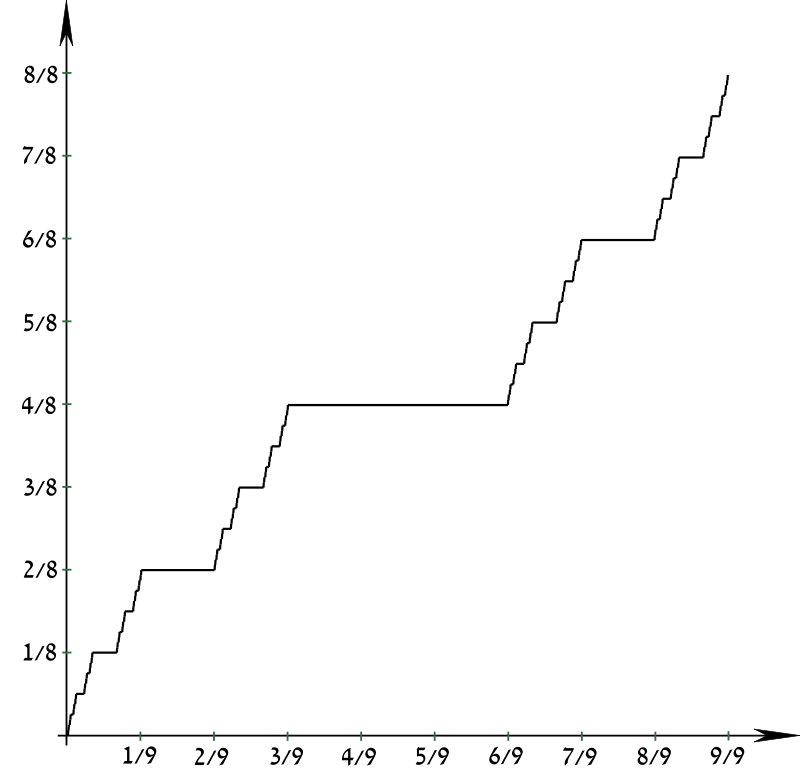
\includegraphics[scale = 0.3]{figure/Cantor_function.png}
    \caption{康托-勒贝格函数示意图}
    %\label{fig:my_label}
\end{figure}
\begin{exercise}
    计算
    \begin{enumerate}
    \item $F(5/12)$, 
    \item $F(4/27), F(22/27)$.
    \end{enumerate}
\end{exercise}
接下来的练习将在例 \ref{Cantor_measure} 中用到. 
\begin{exercise}\footnote{本练习灵感来自B站用户MatPopLeaSpo, UID: 391248289}
    证明: 当$x \in [0,1] \setminus \calC$时, 
    $$ F(1-x) = \sup_{\substack{y \geq x \\ y \in \calC}} F(1-y) = 
    \inf_{\substack{y \leq x \\ y \in \calC}} F(1-y). $$
\end{exercise}
\begin{proof}
    首先完全按照定义, 有
    $\displaystyle{F(1-x) = \sup_{\substack{y \leq 1-x \\ y \in \calC}} F(y)} $. 对$y-1$用换元法得
    $$F(1-x) = \sup_{\substack{y \geq x \\ y \in \calC}} F(1-y). $$
    设$\eps > 0$. 因为$F$在$1-x$处连续, 则存在$\delta>0$, 对所有$1-y_1 \in [1-x, 1-x+\d)$以及$1-y_2 \in (1-x-\d, 1-x]$, 有
    $$ |F(1-y_1) - F(1-y_2)| < \eps. $$
    注意到$1-y_1$和$1-y_2$的取法等价于
    $$ x-\d \leq y_1 \leq x, \quad x \leq y_2 \leq x+\d. $$
    再由$F(1-t)$是关于$t$的单调递减函数, 得
    $$ \sup_{\substack{y \geq x \\ y \in \calC}} F(1-y) = 
    \sup_{\substack{x+\d \geq y \geq x \\ y \in \calC}} F(1-y), \quad
    \inf_{\substack{y \leq x }} F(1-y) = 
    \inf_{\substack{x-\d \leq y \leq x \\ y \in \calC}} F(1-y). $$
    现在对$|F(1-y_1)-F(1-y_2)| < \eps$中的$y_2$取上确界, 得
    $$ |F(1-y_1) -  \sup_{\substack{y \geq x \\ y \in \calC}} F(1-y)| \leq \eps. $$ 再对$y_1$取下确界, 得
    $$|\inf_{\substack{y \leq x \\ y \in \calC}} F(1-y) -  \sup_{\substack{y \geq x \\ y \in \calC}} F(1-y)| \leq \eps. $$
    由于$\eps$是任取的, 且上式中的上下确界与$\eps$无关, 所以
    $$ \sup_{\substack{y \geq x \\ y \in \calC}} F(1-y) = 
    \inf_{\substack{y \leq x \\ y \in \calC}} F(1-y). $$ \qed     
\end{proof}
\begin{example}[~(预告)]
    本例会用不严格的语言描述一下康托-勒贝格函数的一个有趣的性质.
    $F$在$[0,1]\setminus \calC$上是分段常值函数, 所以导数为$0$. 而$m(\calC) = 0$, 所以$F'$几乎处处等于$0$. 但是$F$的图像与$x$轴围成的面积显然$>0$, 也就是说, 微积分中的牛顿-莱布尼茨公式不成立!
    $$\int_0^1 F'(x)~dx = \int_0^1 0~dx = 0. $$
    但是, 勒贝格微积分基本定理能够解释这个问题. 
\end{example}


\subsection{广义康托集及其应用}
康托集的构造过程很容易推广: 改一改挖掉的区间数, 改一改挖去的区间长度,
或者将康托集的一些性质归纳出来进行排列组合, 比如``完全不连通的紧集"等等. 我们也可以将这些集合归于类康托集. 为和正课讲义保持一致, 我们将上面这两种集合统称为``广义康托集". 

\begin{example}\footnote{Real Analysis, Stein, Exercise 1.3}
    设$\xi \in (0, 1)$, 这是我们挖去区间的长度($\xi = 1/3$对应的是康托集). 现在, 我们构造一个广义康托集. 为叙述方便, 我们定义$[a,b](a,b \geq 0)$的长度为$\xi$的\textbf{中心区间}为$$\displaystyle{\left[\frac{a+b}{2}-\frac{\xi}{2}, \frac{a+b}{2} + \frac{\xi}{2} \right]}, $$ 这就是一个以$[a,b]$的中点为中心, $\xi$为长度的区间.  \\
    \textbf{第1步}: 从$[0,1]$中删去长度为$\xi$的中心区间. 记余下的集合为$C_1$. \\
    \textbf{第2步}: $C_1$是两个闭区间的并. 从每个闭区间中删去相对长度\footnote{由于$\xi \in (0,1)$, 所以可以将其理解为所占单位区间的百分比. 若$I$对闭区间$[a,b]$具有相对长度$\xi$, 则$I$的长度为$(b-a)\xi$. }为$\xi$的中心区间, 余下的集合记作$C_2$. \\
    依此类推, 记$\calC_\xi = \bCap{n=1}{\infty}C_n$.
    \begin{enumerate}
    \item 证明$m(\calC_\xi^c) = 1$.
    \item 不用第一问, 证明$m^*(\calC_\xi) = 0$. 
    \end{enumerate}
\end{example}
\begin{proof}
    
\end{proof}
\begin{example}
    
\end{example}


\begin{example} % Stein ex 1-20
    举例: $A, B \subset \R$为闭集且$m(A)=m(B)=0$, 但$m(A+B)>0$.
\end{example}
\begin{proof}
    令$A = \calC, B = \calC / 2$. 
    \qed
\end{proof}


\begin{example}
    构造一个博雷尔集$A \subset [0,1]$满足
    $$ 0<m(A \cap I)<m(I) \quad \text{对所有区间}~I \subset [0,1]~\text{都成立}. $$
\end{example}

\begin{exercise}
    构造$f:\R \to \R$, $f$将开集映成开集, 但$f$不是连续函数. 
\end{exercise}




\begin{example}
    构造一个$\R$中的博雷尔集$A$满足
    $$ 0<m(A \cap I)<m(I) \quad \text{对所有区间}~I~\text{都成立}. $$
\end{example}
\begin{solution}
    % 先证明对所有有理区间成立
    %``构造"和``对所有"明示了这道题的难度非同寻常, 我们必须简化``对所有区间"这个条件. 回想有理数集在实数集中的稠密性, 我们可以尝试用有理区间代替所有区间. 如果我们能构造出$A$使结论对所有有理区间都成立, 那么该结论也应该对所有区间都成立. 现在我们来论证这个陈述:

    %设$\Q = \{r_1, r_2, \cdots\}$, 假设我们已经构造出了博雷尔集$A$满足
    %$$0 < m(A \cap (r_i,r_j)) < r_j - r_i \quad \text{对所有}~r_i<r_j~\text{都成立}.$$
    %现任取一区间$I=(a,b)$(只需考虑开区间即可, 为什么?), 则可以找到有理数$a<r_i<r_j<b$. 接下来,
    %\begin{align*}
    %m(A \cap I)
    %&= m(A \cap (a,r_i)) + m(A \cap (r_i,r_j)) + m(A \cap (r_j,b)) \\
    %&< (r_i-a) + (r_j - r_i) + (b-r_j) \\
    %&= b-a,
    %\end{align*}
    %且$m(A \cap I) \geq m(A \cap (r_i-r_j)) > 0$, 故结论对所有区间$I$都成立. 

    %至此, 我们已将题目简化为了``构造一个$\R$中的博雷尔集$A$满足$0<m(A \cap I)<m(I)$对所有有理区间$I$都成立."
    
\end{solution}

% https://www.jstor.org/stable/pdf/2975692.pdf?refreqid=excelsior%3A200cfff310a747c5a4b7f4620fd7f019&ab_segments=&origin=&acceptTC=1